\openingarticle
\def\ppages{\pagerange{Pasch:firstpage}{Pasch:lastpage}}
\def\shorttitle{Interview: Brian Fagan}
\def\maintitle{Brian Fagan, Ph.D. \textit{Professor Emeritus at the University of California, Santa Barbara}}
\def\shortauthor{Chelsea Colwell-Pasch}
\def\authormail{Chelsea.Colwell-Pasch@gnb.ca}
\def\affiliation{Department of Archaeology, Flinders University, Adelaide, Australia; \\ \noindent Archaeological Services Unit, Fredericton, New Brunswick, Canada}
%--------------------------------------------------------------
\mychapter{Brian Fagan, Ph.D. \textit{Professor Emeritus\\ at the University of California, Santa Barbara}}
\begin{center}
	{\Large\scshape\shortauthor}\\[1em]
	\email \\
	\affiliation
\end{center}
\vspace{3em}
\midarticle
%--------------------------------------------------------------
\label{Pasch:firstpage}
 
\SetBlockThreshold{1} 
\blockquote{This interview was conducted over late May, early June 2015 via email between Dr Fagan and the author for the \textbf{\textit{International Journal of Student Research in Archaeology}}. -- C.~Colwell-Pasch}	
	
	\begin{figure}[!htb]
		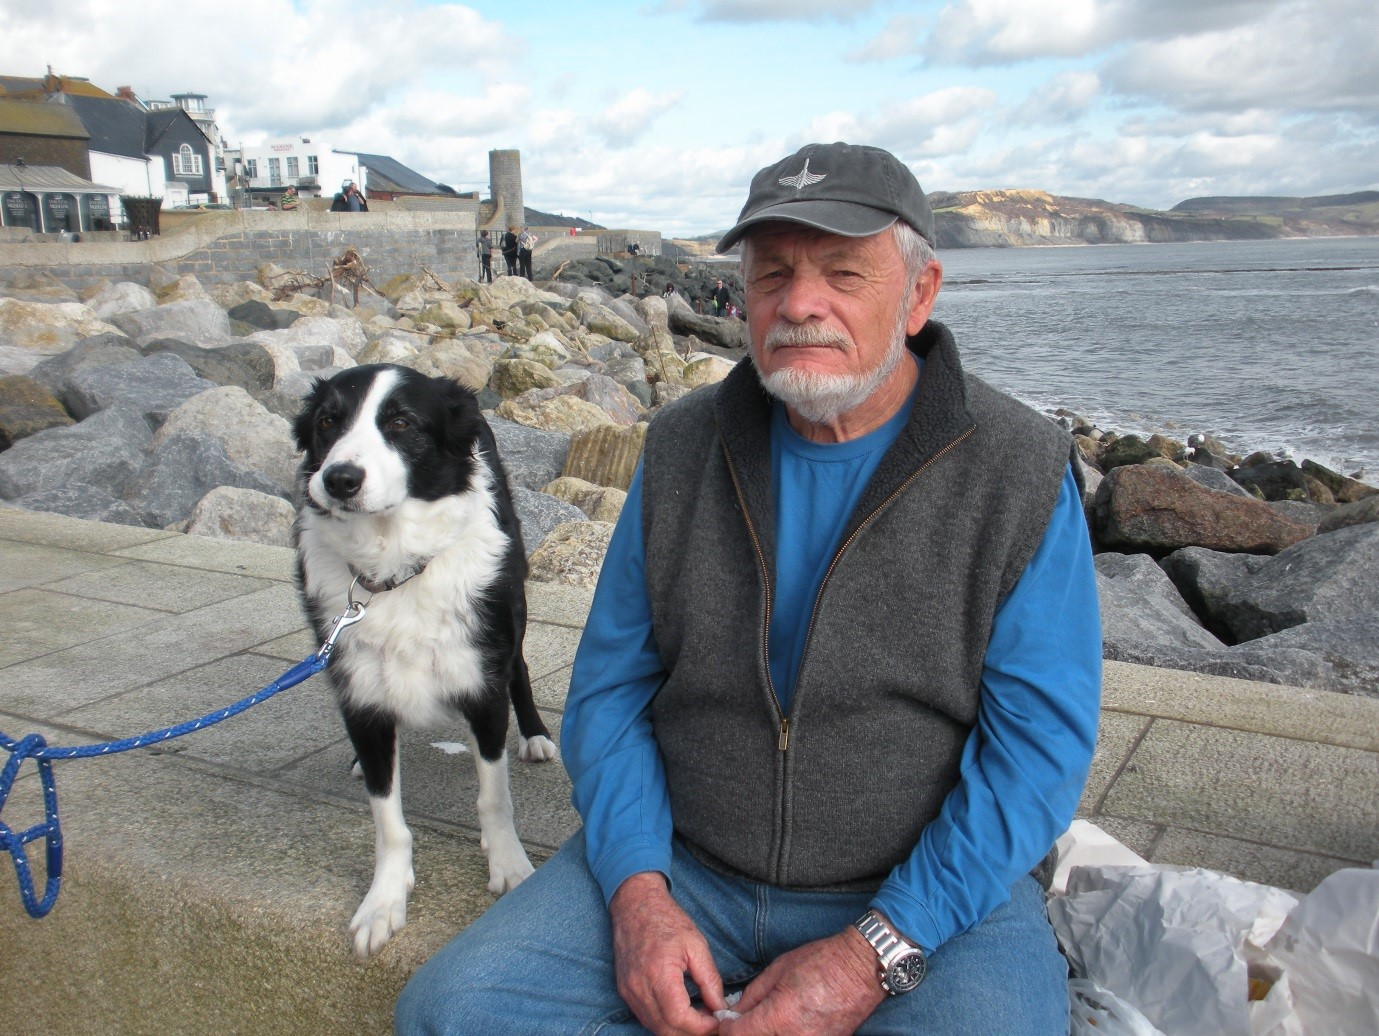
\includegraphics[width=\linewidth]{figures/pasch_Fig1}
		\centering
		\caption{Professor Emeritus Brian M. Fagan with a canine pal. Dr Fagan is an avid animal lover who has three cats and up to 24 rabbits at his home (Photo courtesy of Brian M. Fagan).}
		\label{fig:pasch_Fig1}
	\end{figure}
	
\begin{labeling}{IJSRA}	
\item[IJSRA (International Journal of Student Research in Archaeology)] \textit{Thank you Dr Fagan for allowing IJSRA to interview you for the inaugural issue of our Journal. Your contributions to archaeology are numerous and especially significant for students who are first introduced to archaeology through your foundational texts like} ‘Archaeology: A Brief Introduction’ \textit{(1978), now in its 10th edition. \newline
How did you end up studying archaeology at Cambridge?}
	
\item[BMF (Dr. Brian M Fagan)] I became interested in archaeology at Cambridge University, having elected to study the subject on the recommendation of my tutor. My first instructor was the Stone Age archaeologist, Miles Burkitt, and I got hooked by his story telling. So I stayed on with archaeology for Part II of the degree and specialized in Stone Age archaeology under Charles McBurney.

\item[IJSRA]\textit{Was it a childhood dream or did you happen to “fall into it” as they say?}

\item[BMF] I had no intention of becoming an archaeologist, but met J. Desmond Clark, the Africanist, by chance, and ended up joining the Rhodes-Livingstone Museum in then Northern Rhodesia as Keeper of Prehistory. He was the Director. My mandate was to study the Iron Age cultures of the territory, 100- miles long and 1,000 wide, which is the history and archaeology of the modern African inhabitants. This got me in on the ground floor of multidisciplinary African history.

\item[IJSRA]\textit{What do archaeology students today have to face that is different from your generation?}

\item[BMF] When I entered the field, archaeology was expanding, especially in the US and overseas. We were encouraged to work abroad by Grahame Clark, the Professor of the day at Cambridge. Few of us had PhDs, but sometimes acquired them in later years, as I did. Archaeology really was a village in those days and one tended to have met most people. There were plenty of jobs, especially if you were prepared to leave Britain, mainly in what was then the British Empire. Today, we’re paying the price of too rapid expansion, gross-overproduction of PhDs, and training that is ever more specialized and high-tech. That makes it hard for many people to launch careers, especially when many folk are retiring later.
	
\item[IJSRA]\textit{You mentioned on your website that you had almost given up archaeology in 1966 before changing roles from specialist to generalist.  What roles do specialisations have in archaeology today, and if a student wanted to specialise in something specific what would your advice be?}

\item[BMF] We live in a world of specialisations, and the problem is not facing archaeology alone. One factor is the “publish or perish” syndrome, another the overproduction of PhD students, many of whom follow in their already specialised mentor’s footsteps. To be employable in most of higher education today, you have to be; (a) possessing of a broad general knowledge of archaeology to teach internationally minded students, (b) able to teach well at the undergraduate level, and (c) have a strong multidisciplinary perspective. If you are going to specialise, go into something with an ingrained multidisciplinary perspective, be prepared to be part of a research team, and try and acquire an expertise in something that has a relevance to today’s world. Cultural resource management and heritage are still expanding areas, especially the latter and cultural tourism. Be aware that you cannot become a credible generalist without having some fieldwork and some specialized archaeology; also to have published it.	

\item[IJSRA]\textit{You were the “Keeper of Prehistory” at the Livingstone Museum in Zambia, Central Africa in the 1960’s. Do you feel colonialism played or plays a role (good or bad) in fostering archaeological research and influencing archaeological interpretation in less developed regions?}

\item[BMF] No question that “colonialism” played a role in fostering archaeological research. Apart from early human evolution, a main thrust while I was in Africa was developing multidisciplinary history in which archaeology played a major role. Our research went straight into school and university curricula. There was nothing else. Colonial administrators did much to foster museums and monuments protection. They were, on the whole, a benign influence culturally, except in post-independence Rhodesia and South Africa. The controversies over ‘Great Zimbabwe’ are a classic example of colonial interference.

\item[IJSRA] \textit{What is the motivation and impact of post-colonial theory in archaeological research and interpretation?}

\item[BMF] I do not know how to answer this question, as I no longer work in Africa. My impression of the field is that it has moved well ahead of that. Sorry. Not my expertise. But they are still writing history, much of the emphasis being local, I think.

\item[IJSRA] \textit{What can we learn from the historic background of the development of the discipline?}

\item[BMF] Any discipline is a product of its history, and archaeology is no exception. We learn a great deal from the mistakes and challenges faced by our predecessors, who were poorly funded, and very thin on the ground. It’s remarkable what they achieved and we have much to learn from them, so we don’t reinvent the wheel.

\item[IJSRA] \textit{You were appointed to the University of California – Santa Barbara in 1967. How are approaches in archaeological research, teaching, and funding different in the US compared to the UK?}

\item[BMF] Undergraduate education in the US is on an enormous scale with many anthropology classes with over 1,000 students. The largest introductory archaeology classes were, in my day, about 300, which was bad enough. There is a huge emphasis on testing and grading, which is mindless nonsense, and in my view, counterproductive. I think the UK system with its essays and annual exams is much better, for it forces students to take responsibility for their work and to think. The total obsession in academic archaeology these days is ‘publish or perish’, with there being intense competition for permanent jobs. Many instructors are now on short-term contracts as a way of saving money, which is a dreadful way to build a career, and are underpaid. At major research universities, there is a great preoccupation with fund raising and money and you get rewarded for the grants you obtain. Not a healthy way to advance knowledge.

\item[IJSRA] \textit{How do you feel the social engagement with archaeology of the British population differs in comparison to the US, and indeed on a more global scale?}
	
\item[BMF] I would say that the US population as a whole is little engaged in archaeology. It being generally the archaeology of “them” (Native Americans), rather than “us”. There is, of course, stronger interest in historical archaeology, the period after 1492. Archaeology is much more embedded in the UK mind, largely because of TV, most recently ‘Time Team’. Globally, the interest varies wildly. Oddly enough, the Germans are very interested in Native Americans. Scandinavia is seriously engaged with the remote past.
	
\item[IJSRA] \textit{You have worked as a consultant with various organisations throughout your career, like National Geographic. What are the opportunities/limitations for engaging with non-archaeological organisations?}

\item[BMF] Opportunities to engage with non-archaeological organizations depend entirely on individual initiative. There’s an open demand for lectures from local organizations of all kinds. Major keynotes and other platforms are few and far between. Generally non-archaeological organizations recruit people who have written general books of broad interest. I would say that about 50\% of my lecturing is for non-archaeological audiences, which appears to be unusually high. A word to the wise: It’s fatal to assume that everyone is interested in archaeology. They aren’t.
                
\item[IJSRA] \textit{You were awarded the Society of Professional Archaeologists' ‘Distinguished Service Award’ in 1996 for your "untiring efforts to bring archaeology in front of the public." How important is public/community engagement within archaeology?}

\item[BMF] Engagement with the public is all-important in an era of unprecedented destruction of archaeological sites worldwide. And it’s a time when funding shortfalls are making people, especially politicians, think about priorities. How does archaeology rank against such issues as social safety nets, environment, poverty, and national defence, as well as restoring infrastructure? We definitely have a perception problem; many people still think archaeology is a self-indulgent activity. And in some cases, I’m afraid they’re right. We cannot afford to be an ivory-tower discipline divorced from the real world. This is one of the great challenges for future generations of archaeologists.

\item[IJSRA] \textit{Also in 1996 you received a ‘Presidential Citation Award’ from the Society for American Archaeology (SAA) for your work in textbook, general writing and media activities. What is the role of publishing archaeological research, and what is the point of publishing “for the public”, rather than (or in addition to) a specialised, academic audience?}

\item[BMF] It’s important to make sure that archaeology reaches as broad an audience as possible if it is to survive in the future. As part of this effort, publishing books and articles for a general audiences is all-important, something that is getting harder and harder in a world saturated with books (often junk ones) and other, including electronic, media. It’s very important that we publish first rate material for general audiences and that we tell good stories based on solid science that are compelling, relevant, and entertaining.

\item[IJSRA] \textit{You mentioned we cannot be an “ivory tower discipline.” Do you believe there is still an “ivory tower” separating the public from archaeological research?}

\item[BMF] Yes, although it’s more permeable. To put it grossly simplistically, the priorities of much of academia are raising money and publication and increasingly specialized research—very pervasive values in today’s research universities. And these priorities are not only wrong, they are inappropriate for a discipline like archaeology, which, as Barry Cunliffe once somewhat aptly remarked, “is really a series of unperformed theatrical performances”.

\item[IJSRA] \textit{Should students get involved in the publication and the dissemination of archaeological knowledge, or are top academics better positioned for doing this kind of work?}

\item[BMF] Yes, they should be, for the earlier you start the longer and better your experience, especially in the areas of writing for general audiences and fluent public speaking. As I said before, it is hard, if not impossible, to do this without solid first-hand archaeological experience. It is definitely not something for only senior folk to undertake. Quite the contrary.
	
\item[IJSRA] \textit{Many of your recent books, like} ‘The Long Summer’ \textit{(2004) and} ‘Elixir: A History of Water and Humankind’ \textit{(2011) have a focus on climate change and sea level rise. How do you feel archaeology plays a role in understanding these phenomena and why should future archaeologists understand these contemporary issues?}
                
\item[BMF] Climate change, sustainability, water, whatever… it’s vital that archaeology concern itself with today’s world. There are many perceptions and ideas from the past that have relevance today. Of course, to say that we are destined to repeat the mistakes of history is an oversimplification, for the world has changed so drastically in recent decades. But we have a huge amount to tell today’s world about cultural and biological diversity, and about the nature of being human.

\item[IJSRA] \textit{IJSRA is a student run and student research focused international peer-reviewed journal. Do you believe that students can contribute to international dialogues and perspectives on archaeology with a value equal to those with higher degrees?}

\item[BMF] I think it’s very important that students, as the future generation, contribute to the international dialogue. This is how something like archaeology retains its vitality. Without new ideas, fresh faces, and innovative perspectives, we are nothing.

\item[IJSRA] \textit{Do you have any advice or wisdom you would like to impart on those who are choosing to enter archaeology as a career, either professionally or in academia?}

\item[BMF]Be multidisciplinary, work in areas unexplored by others, and don’t consider archaeology as a career unless you have a passion for it, fire in your belly if you will. It’s not for everyone. And if, after a few years, you find you aren’t happy, get out while the going’s good. I know a large number of middle-aged (and older) archaeologists who have regrets. On another note, there are hundreds of archaeologists who spend their entire careers studying deliciously obscure, high specialised topics and publishing their work for fewer than half a dozen people. This is fine, but it’s a form of scholarship in archaeology that may be endangered by budget cuts. Now there’s a provocative statement to end with!           

  \end{labeling}
\noindent\rule[0.5ex]{\linewidth}{1pt}

\SetBlockThreshold{1} 
\blockquote{Dr Brian Fagan is a prolific author of popular and generalist archaeology books and Professor Emeritus at the University of California, Santa Barbara where he served as Professor of Anthropology from 1967 to 2003. Dr Fagan trained in archaeology and anthropology at Pembroke College, Cambridge, in his native England (BA - Honours 1959, MA 1962, PhD 1964). After spending six years as ‘Keeper of Prehistory’ at the Livingstone Museum in Zambia, Central Africa, he moved to the United States of America in 1966 and decided to completely change the focus of his career. Dr Fagan was a specialist in African Iron Age archaeology, but decided to switch his concentration to communicating archaeology. His talent for simple and effective communication of complex topics has led Dr Fagan to write and edit 46 books, including seven popular undergraduate texts that are many archaeologists’ introduction to the field. He has also published over 100 specialist and generalist peer-reviewed papers.}



	\label{Pasch:lastpage}
\closingarticle